\documentclass{article}



% lua
\label{pkg: luacode}
\usepackage{luacode}



% xparse - multiple optional arguments
\label{pkg: xparse}
\usepackage{xparse}



% Geometry
\label{pkg: geometry}
\usepackage{geometry}
\geometry{
	papersize=	{180mm, 240mm},	% ( 4:3 )	SVGA x 0.3
	top=		.12\paperheight,
	bottom=		.12\paperheight,
	left=		.06\paperwidth,
	right=		.06\paperwidth,
	portrait=	true,
}
%	papersize=	{300mm, 400mm},	% ( 4:3 )	SVGA x 0.5
%	papersize=	{240mm, 320mm},	% ( 4:3 )	SVGA x 0.4
%	papersize=	{180mm, 240mm},	% ( 4:3 )	SVGA x 0.3
%	papersize=	{229mm, 305mm},	% ( 4:3 )	ArchA/Arch1
%	papersize=	{320mm, 512mm},	% (16:10)
%	papersize=	{280mm, 448mm},	% (16:10)
%	papersize=	{240mm, 384mm},	% (16:10)
%	a4paper, %	{210mm, 297mm},	% (√2:1)	A4



% Font size
\label{pkg: fontsize}
\usepackage[fontsize=12pt]{fontsize}



% Linguagem
\label{pkg: babel}
\usepackage[portuguese]{babel}	% Babel
%\usepackage{polyglossia}		% Polyglossia
%\setdefaultlanguage[variant=brazilian]{portuguese}



% Graphics
\label{pkg: graphics}
\usepackage
	[
%		draft,
%		final,
	]
	{
		graphics	% simple
%		graphicx	% extended
	}
\graphicspath{{./images}}



% calc
\label{pkg: calc}
\usepackage{calc}



% Table of contents
\label{pkg: tocloft}
\usepackage{tocloft}
\setcounter{tocdepth}{2}	% remove subsubsection from toc

% part
\renewcommand\cftpartfont{\bfseries}
%\renewcommand\cftpartafterpnum{\vspace{0mm}}
\setlength\cftbeforepartskip{6mm}

% sec
\renewcommand\cftsecfont{\bfseries}	% Font
\renewcommand\cftsecpagefont{}	% page number font
\renewcommand\cftsecleader{\cftdotfill{\cftdotsep}}	% Dots
\setlength\cftbeforesecskip{3mm}
\setlength\cftsecindent{0mm}
%\setlength{\cftsecnumwidth}{25mm}	% Fix section width

% subsec
\setlength\cftsubsecindent{0mm}
%\setlength{\cftsubsecnumwidth}{15mm}

% tab (table)
\setlength\cfttabindent{0mm}



% filecontents
\label{pkg: scontents, filecontents}
%\usepackage{scontents}		% the better filecontents
%\usepackage{filecontents}	% Create files



% Multicols
\label{pkg: multicol}
\usepackage{multicol}
\setlength{\columnsep}{.05\textwidth}



% enumitem
\label{pkg: enumitem}
%\usepackage{enumitem}	% modify enumerate index



% titlesec
\label{pkg: titlesec}
%\usepackage{titlesec}
%
%% Part customization
%\titleclass{\part}{straight}
%\titleformat{\part}
%	[block]							% shape
%	{\huge\bfseries\color{Emph}}	% format
%	{\thepart\hspace{5mm}{$|$}}		% label
%	{5mm}							% sep
%	{\huge\bfseries}				% before-code
%	[\vspace{0.5mm}]				% after-code
%\counterwithin*{section}{part}		% Reset section on part
%\@addtoreset{section}{part}
%
%% Chapter customization
%\titleclass{\chapter}{straight}
%\titleformat{\chapter}
%	[block]
%	{\Huge\bfseries\color{Emph}}
%	{\thechapter\hspace{5mm}{$|$}}
%	{5mm}
%	{\Huge\bfseries}
%	[\vspace{0.5mm}]



% Appendix
\label{pkg: appendix}
%\usepackage{appendix}



% siunix: SI units
\label{pkg: siunitx}
%\usepackage{siunitx}
%	\sisetup{
%		% scientific / engineering / false / fixed
%		scientific-notation =	engineering,
%		exponent-to-prefix =	true,			% 1000 g -> 1 kg
%		exponent-product =		*,				% x * 10^y
%		round-mode =			places,			% figures/places/off
%		round-precision =		2,
%	%	round-minimum =			0.01,
%	%	fixed-exponent =		0,
%	}
%	\DeclareSIUnit\atm{atm}
%	\DeclareSIUnit\calorie{cal}



% Maths
\label{pkg: amsmath, amssymb, bm}
%\usepackage{amsmath, amssymb, bm}
%\usepackage{derivative}		% Derivative
%% Missing trigonometric math operators
%\DeclareMathOperator{\arcsec}{arcsec}
%\DeclareMathOperator{\arccot}{arccot}
%\DeclareMathOperator{\arccsc}{arccsc}
%
%% BM
%\NewDocumentEnvironment{BM}{ O{\large} O{align*} +b }
%{
%	#1\boldmath\bfseries
%	\begin{#2}
%		#3
%	\end{#2}\relax
%} {\relax}
%
%% BM old
%%\newcommand{\BM}[1]{{\large\boldmath\bfseries%
%%	\begin{align*}
%%		#1
%%	\end{align*}%
%%}}
%
%\newcommand\vizinhanca[2][\delta]{%
%	\hyperref[vizinhanca]{V_{#1}(#2)}%
%}
%
%\newcommand\converge{{\,\xrightarrow{\text{converge}}\,}}



% Vectors
\label{pkg: esvect}
%\usepackage{esvect} 	% Vector over-arrow
%\renewcommand{\vec}{\vv} % Vecto over-arrow



% Tikz
\label{pkg: tikz}
%\usepackage{tikz}
%\usepackage{pgfmath}	% calculations
%\usepackage{varwidth}	% List inside TikzPicture


% pgf
% pgfmath
\label{pkg: pgfmath}
%\usepackage{pgfmath}	% calculations
%
% pgfplots
\label{pkg: pgfplots}
%\usepackage{pgfplots}
%	\pgfplotsset
%	{
%		compat= newest,
%		width=	.90\linewidth,	% width
%		height=	.22\textheight,	% height
%		legend style=
%		{
%			draw=	none,
%			fill=	White\Dark,
%			fill opacity=	0.3,
%			text opacity=	1,
%		},
%		major grid style=
%		{
%			very thin, 
%			color= White!60!Black
%		},
%		ticklabel style=
%		{
%			/pgf/number format/.cd,
%			set thousands separator={\,},
%			tick style= {color= White!60!Black},
%		},
%		every extra x tick/.style=
%		{
%			tick style= {draw=none},
%			major grid style=
%				{ draw, thin, color= White!90!Black },
%			ticklabel pos= top,
%		},
%		every extra y tick/.style=
%		{
%			tick style= {draw=none},
%			major grid style=
%				{ draw, thin, color= White!90!Black },
%			ticklabel pos= right,
%		},
%	}
%
% pgfplotstable
\label{pkg: pgfplotstable}
%\usepackage{pgfplotstable}



% Tabular
\label{pkg: multirow, float, longtable}
%\usepackage{multirow}
%\usepackage{float}	% table position H(ere)
%	\restylefloat{table}
%\usepackage{longtable}
%
%\setlength\tabcolsep{6mm}			% width
%\renewcommand\arraystretch{1.25}	% height
%
% booktabs
\label{pkg: booktabs}
%\usepackage{booktabs}
%\setlength\heavyrulewidth{.75pt}	% Top and bottom rule
%\setlength\lightrulewidth{.50pt}	% Middle rule
%\usepackage{colortbl}				% Colored Cells



% Chem
\label{pkg: chemformula, chemfig, modiagram}
%\usepackage{chemformula}	% formulas quimicas
%\usepackage{chemfig}		% Estruturas quimicas
%\usepackage{modiagram}		% Molecular orbital diagram
%	\setmodiagram
%	{
%		names,
%		labels,
%		labels-fs=\tiny,	% label font
%		AO-width=6mm,
%	}
%
%\newcommand{\mol}[1]{ \unit{\mole\of{\ch{ #1 }}} } % mol



% Constants
\label{pkg: physconst, physunits}
%\usepackage{physconst, physunits}



% Code
\label{pkg: shellesc, minted}
% Run on terminal: lualatex --shell-escape [file[.tex]]
\usepackage{shellesc, minted}
	\setminted
	{
		linenos,		% line number
		autogobble,		% line trim
		tabsize= 4,		% tab size
		obeytabs,		% tab alignment
		breaklines,		% break lines
%		python3,		% Python lexer or idk
	}
	\usemintedstyle{stata-dark}
%	\usemintedstyle{fruity}
%	\usemintedstyle{paraiso}
%	\usemintedstyle{rainbow_dash}
%	\usemintedstyle{solarized-dark}
%	\usemintedstyle{native}



% Colors
\label{pkg: xcolor}
\usepackage{xcolor}

\definecolor{DarkBlue}  {HTML}{252A36}
\definecolor{LightGreen}{HTML}{7CCC6C}
\definecolor{DarkGreen} {HTML}{008675}

\colorlet{White}{DarkGreen!20}
\colorlet{Black}{DarkBlue!110}
%\colorlet{Black}{DarkBlue!70!black}
\colorlet{Emph}{ DarkGreen!70!White}
\colorlet{Background}{White!40!Black}

\pagecolor{Black}
\color{White}

%% mycolors
%% Pallete
%\definecolor{red}   {HTML}{FF0000}
%\definecolor{orange}{HTML}{FF7300}
%\definecolor{yellow}{HTML}{FFEA00}
%\definecolor{green} {HTML}{2AFF00}
%\definecolor{cyan}  {HTML}{00FFBF}
%\definecolor{blue}  {HTML}{0055FF}
%\definecolor{purple}{HTML}{9500FF}
%\definecolor{pink}  {HTML}{FF0080}
%% Light
%\newcommand\Light{!63!White}
%\colorlet{Red}   {red\Light}
%\colorlet{Orange}{orange\Light}
%\colorlet{Yellow}{yellow\Light}
%\colorlet{Green} {green\Light}
%\colorlet{Cyan}  {cyan\Light}
%\colorlet{Blue}  {blue\Light}
%\colorlet{Purple}{purple\Light}
%\colorlet{Pink}  {pink\Light}
%% Dark
%\newcommand\Dark{!45!Black}
%\colorlet{DRed}   {Red\Dark}
%\colorlet{DOrange}{Orange\Dark}
%\colorlet{DYellow}{Yellow\Dark}
%\colorlet{DGreen} {Green\Dark}
%\colorlet{DCyan}  {Cyan\Dark}
%\colorlet{DBlue}  {Blue\Dark}
%\colorlet{DPurple}{Purple\Dark}
%\colorlet{DPink}  {Pink\Dark}



% tcolorbox
\label{pkg: tcolorbox}
\usepackage{tcolorbox}
	\tcbuselibrary%
	{
		breakable,					% allow page break
		minted, xparse, listings,	% code minted
	}
	\tcbset%
	{	every box/.style= {
		coltext=		White,		% text  color
		coltitle=		White,		% title color
		fonttitle=		\bfseries,	% title font
		opacityfill=	0.1,		% background opacity
		opacityframe=	0,			% frame      opacity
		colback=		Background, % background color
		colframe=		Background,	% border     color
		arc=			3mm,		% Curvature
		width=			\linewidth,	% Width
	}}



% mytitle and myauthor
\label{Set: title, author}
\newcommand\mytitle{{ICE-B - Teste 2}}
\newcommand\myauthor{{Felipe B. Pinto 61387 - MIEQB}}



% title, author and date
\title{\huge\bfseries\color{Emph}\mytitle}
\author{\Large\myauthor}
\date{\Large\today}



% fancyhdr - Header and Footer customization
\label{pkg: fancyhdr}
\usepackage{fancyhdr}
	\pagestyle{fancy}
	\lhead{\normalsize\myauthor}
	\rhead{\normalsize\today}



% hyperref
\label{pkg: hyperref}
\usepackage{hyperref}
	\hypersetup
	{
		% Links customization
		hidelinks=true,
		colorlinks=true,
		linkcolor=LightGreen!25!White,
		% PDF customization
		pdfpagelayout=OneColumn,
		pdftitle=\mytitle,
		pdfauthor=\myauthor
	}
% Fix links when reseting section on part
\renewcommand\theHsection{\thepart.\thesection}



% questions, subquestions and subsubquestions
\label{sec: question, subq, subsubq}

% question
\newcounter{question}[part]
\renewcommand{\thequestion}{Questão \arabic{question}}
\newcommand{\question}[1]{
	% reset inner counters
	\setcounter{subquestion}{0}
	\setcounter{subsubquestion}{0}
	% add section*
	\refstepcounter{question}
	\section*{\thequestion\quad#1}
	% add to toc
	\addcontentsline{toc}{section}{%
		\thequestion\quad#1%
	}
}

% subquestion
\newcounter{subquestion}[part]
\renewcommand\thesubquestion{%
	Q\arabic{question} - \alph{subquestion})%
}
\newcommand{\subquestion}[1]{
	% reset inner counters
	\setcounter{subsubquestion}{0}
	% add subsection*
	\refstepcounter{subquestion}
	\subsection*{\thesubquestion\quad#1}
	% add to toc
	\addcontentsline{toc}{subsection}{%
		\thesubquestion\quad#1%
	}
}

% subsubquestion
\newcounter{subsubquestion}[part]
\renewcommand{\thesubsubquestion}{(\roman{subsubquestion})}
\newcommand{\subsubquestion}[1]{
	% add subsubsection*
	\refstepcounter{subsubquestion}
	\subsubsection*{\thesubsubquestion\quad#1}
	% add to toc
	\addcontentsline{toc}{subsubsection}{%
		\thesubsubquestion\quad#1%
	}
}



% Questions environment
\label{env: question, box}

% question
\NewDocumentEnvironment{questionBox}
	{ s t1 t2 t3 O{5mm} m +b }
	{
		\vspace{#5}\relax
		\IfBooleanF{#1}{\noindent\begin{minipage}{\linewidth}}
			\IfBooleanT{#2}{      \question{#6}\relax}
			\IfBooleanT{#3}{   \subquestion{#6}\relax}
			\IfBooleanT{#4}{\subsubquestion{#6}\relax}
			\begin{tcolorbox} #7 \end{tcolorbox}\relax
		\IfBooleanF{#1}{\end{minipage}\relax}
	} {\relax}

% code
\DeclareTCBListing{codeBox}
	{ s t1 t2 t3 O{5mm} O{left=2.5em} m m }
	{
		\IfBooleanT{#1}{breakable,}%
		before=
		{
			\vspace{#5}
			\IfBooleanF{#1}{\noindent\begin{minipage}}
			\IfBooleanT{#2}{      \question{#8}}
			\IfBooleanT{#3}{   \subquestion{#8}}
			\IfBooleanT{#4}{\subsubquestion{#8}}
		},
		\IfBooleanF{#1}{after= {\end{minipage}},}%
		listing only,
		listing engine= minted,
		minted language= #7,
		minted options={},
		#6
	}



%% Incompleto
%
%% Listoftemas: tema e subtema
%\newlistof{temas}{prog}{}
%%% Add to document
%%\section*{Programa}
%%\begin{multicols}{2} \listoftemas \end{multicols}
%% tema
%\newcounter{tema}[section]
%\newcommand\tema[1]{%
%	\refstepcounter{tema}%
%	\addcontentsline{prog}{temas}{%
%		\thetema\textsuperscript{o} Tema: #1%
%	}%
%}
%% subtema
%\newcounter{subtema}[subsection]
%\newcommand\subtema[1]{%
%	\refstepcounter{subtema}%
%	\addcontentsline{prog}{temas}{%
%		\textbullet\quad#1%
%	}
%}



%% subsubsection customization
%\renewcommand\thesubsubsection{(\roman{subsubsection})}



\begin{document}

\question{}

%\begin{multicols}{2}

\begin{questionBox}2{}
	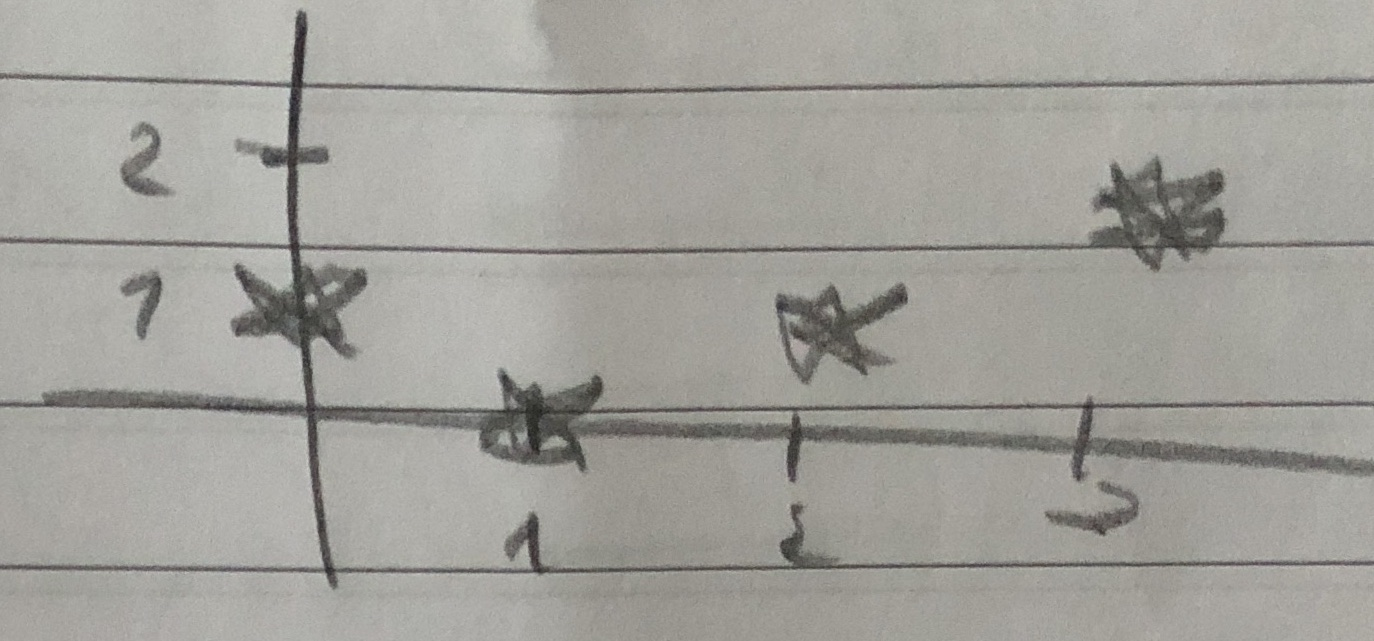
\includegraphics[width=.8\linewidth]{Q1 - a).jpg}
\end{questionBox}

\begin{questionBox}2{}
	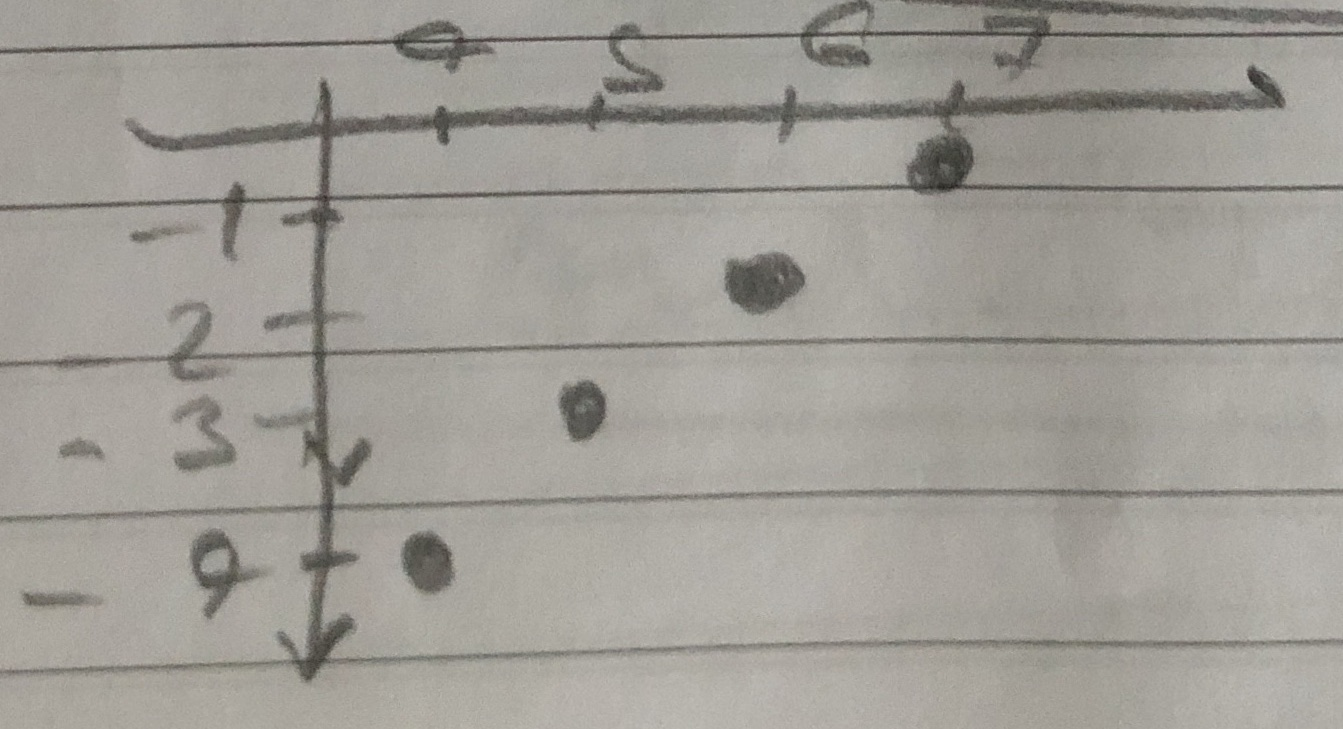
\includegraphics[width=.8\linewidth]{Q1 - b).jpg}
\end{questionBox}

\begin{questionBox}1{}
	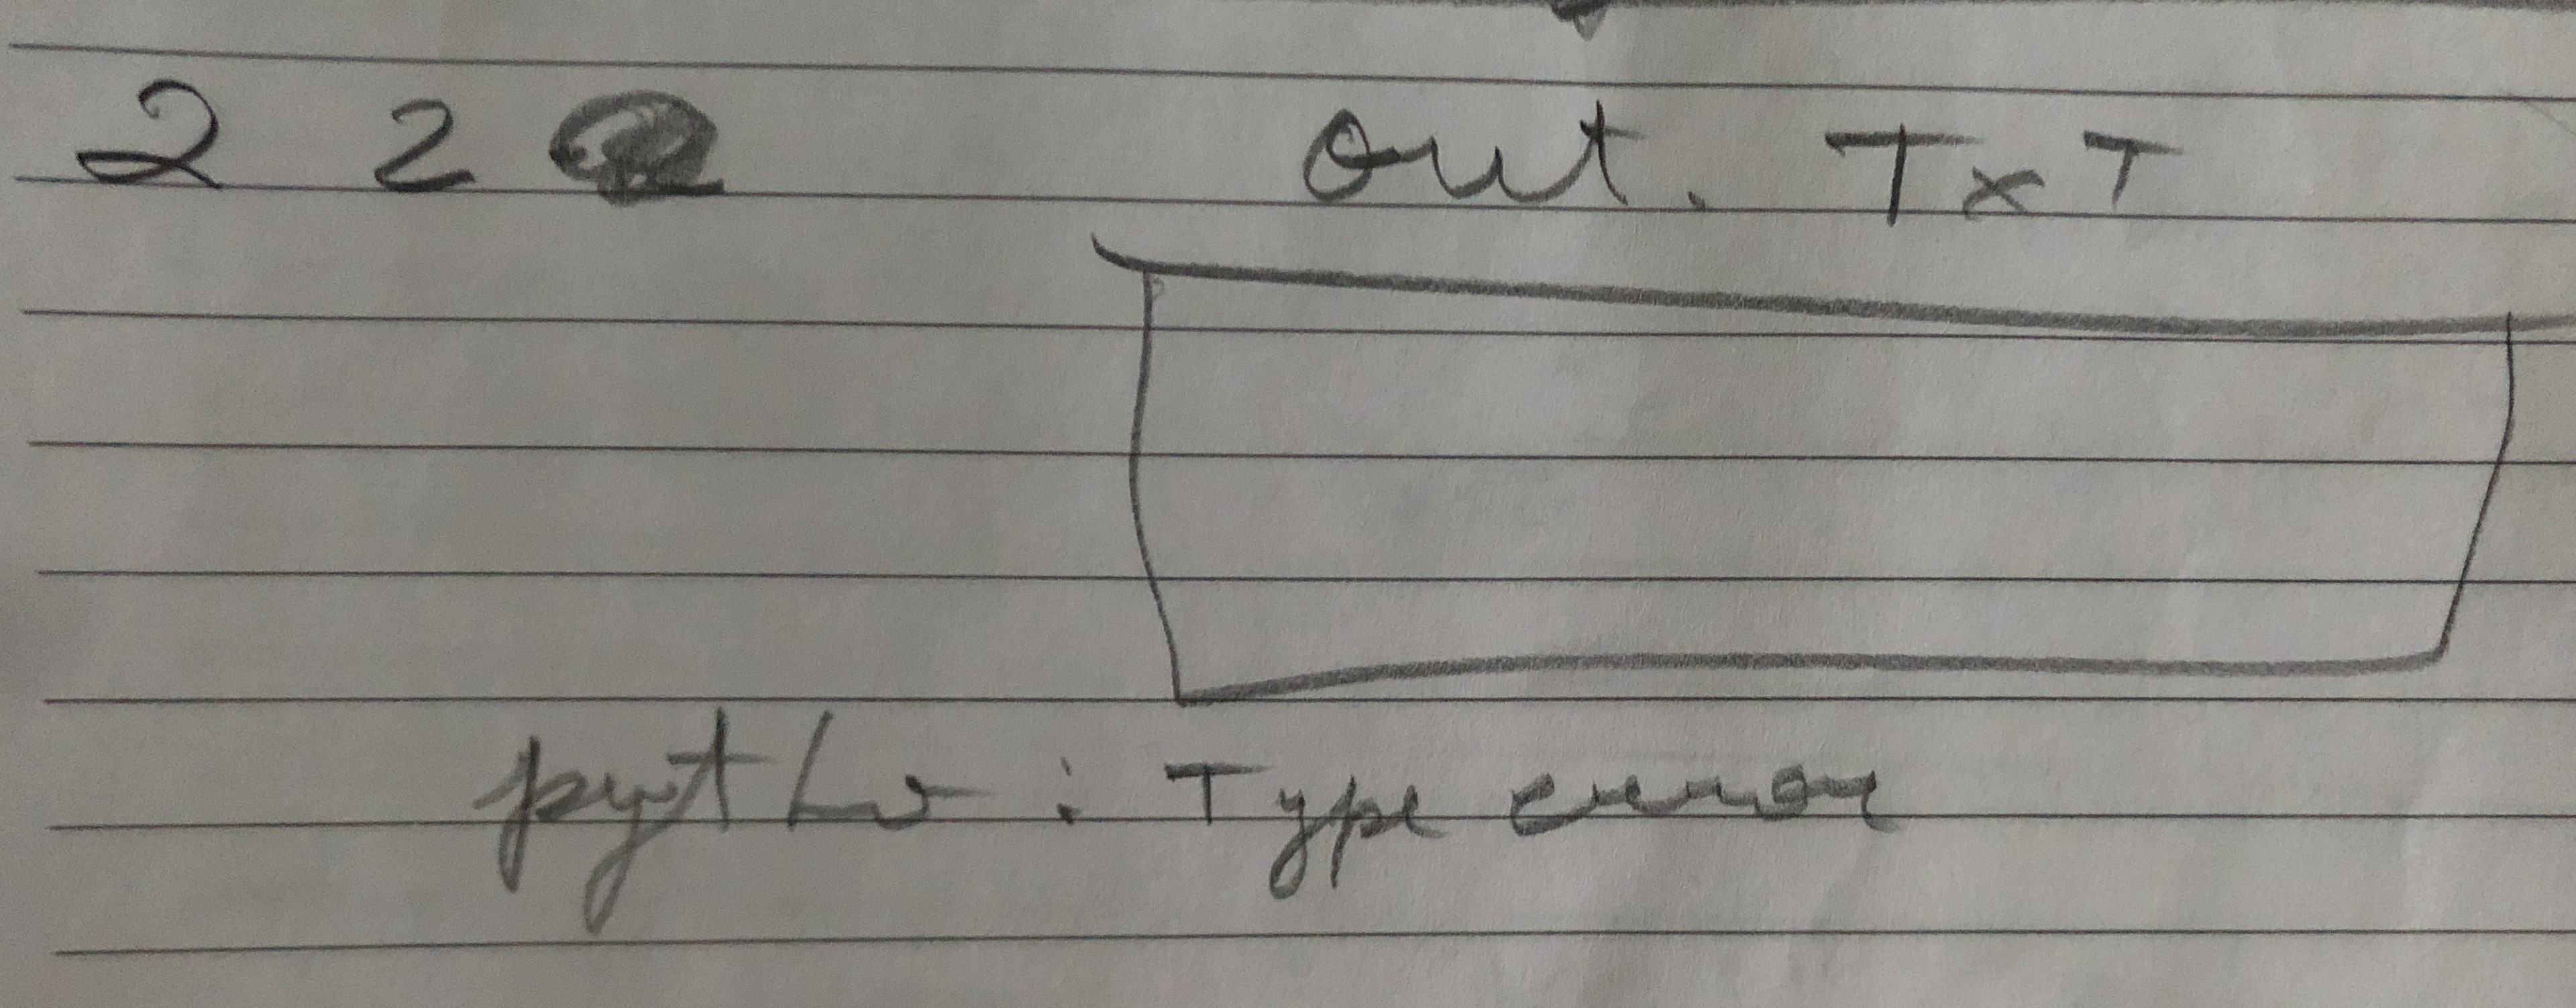
\includegraphics[width=.8\linewidth]{Q2.jpg}\\
	Python: Type error
\end{questionBox}

\vspace{5mm}

\begin{tcblisting}{
	before=%
	{%
		\vspace{5mm}
		\noindent\begin{minipage}{\linewidth}
		\question{}
	},
	after= {\end{minipage}},
	listing only,
	listing engine= minted,
	minted language= python,
	minted options={},
	left=2.5em,
}
L = [
		"smartfone:145"
		"laptop:550"
		"monitor:195"
	]
\end{tcblisting}

\begin{tcblisting}{
	before=%
	{%
		\vspace{5mm}
		\noindent\begin{minipage}{\linewidth}
		\question{}
	},
	after= {\end{minipage}},
	listing only,
	listing engine= minted,
	minted language= python,
	minted options={},
	left=2.5em,
}
	x = "123-smartfone"
	y = "67)"
	v = 67
\end{tcblisting}

\begin{tcblisting}{
	before=%
	{%
		\vspace{5mm}
		\noindent\begin{minipage}{\linewidth}
		\question{}
		\subquestion{}
	},
	after= {\end{minipage}},
	listing only,
	listing engine= minted,
	minted language= python,
	minted options={},
	left=2.5em,
}
	x = (
		("técnico", "Lisboa"),
		("técnico", "Porto"),
		("especialista", "Lisboa")
	)
\end{tcblisting}


\begin{tcblisting}{
	before=%
	{%
		\vspace{5mm}
		\noindent\begin{minipage}{\linewidth}
		\subquestion{}
	},
	after= {\end{minipage}},
	listing only,
	listing engine= minted,
	minted language= python,
	minted options={},
	left=2.5em,
}
	x = (
		("VOS", "Operador", 1217.5),
		("GLP", "Técnico", 1345.9)
	)
\end{tcblisting}


\begin{tcblisting}{
	before=%
	{%
		\vspace{5mm}
		\noindent\begin{minipage}{\linewidth}
		\subquestion{}
	},
	after= {\end{minipage}},
	listing only,
	listing engine= minted,
	minted language= python,
	minted options={},
	left=2.5em,
}
	x = (
		"especialista",
		"operador",
		"técnico"
	)
\end{tcblisting}


\begin{tcblisting}{
	before=%
	{%
		\vspace{5mm}
		\noindent\begin{minipage}{\linewidth}
		\subquestion{}
	},
	after= {\end{minipage}},
	listing only,
	listing engine= minted,
	minted language= python,
	minted options={},
	left=2.5em,
}
	x = (1956.7)
\end{tcblisting}


\begin{tcblisting}{
	before=%
	{%
		\vspace{5mm}
		\noindent\begin{minipage}{\linewidth}
		\subquestion{}
	},
	after= {\end{minipage}},
	listing only,
	listing engine= minted,
	minted language= python,
	minted options={},
	left=2.5em,
}
	com = "SELECT Empresa.nome, Local, Salário FROM Anúncios, Empresas WHERE Empresas.id=Anúncios.emp_id AND Anúncios.Posição=\"Técnico\""
\end{tcblisting}


\begin{tcblisting}
{
	before=%
	{%
		\vspace{5mm}
		\noindent\begin{minipage}{\linewidth}
		\question{}
		\subquestion{}
	},
	after= {\end{minipage}},
	listing only,
	listing engine= minted,
	minted language= python,
	minted options={},
	left=2.5em,
}
def ...(...):
	try: results = q.select(nomeBD, "SELECT Empresas.nome, posição, local FROM Empresas, Anuncios WHERE Empresas.id=Anuncios.emp_id AND Anuncios.salário>=?", min_sal)
	except sqlite.Error: raise
	
	results = [f"{result[0]}:{result[1]}({result[2]})" for result in results]
	
	return results
\end{tcblisting}


\begin{tcblisting}
{
	before=%
	{%
		\vspace{5mm}
		\noindent\begin{minipage}{\linewidth}
		\subquestion{}
	},
	after= {\end{minipage}},
	listing only,
	listing engine= minted,
	minted language= python,
	minted options={},
	left=2.5em,
}
def ...(...):
	results=obtem_registros(nomeBD, min_sal)
	with open(rname,"w") as out:
		for result in results:
			out.write(result)
\end{tcblisting}


\begin{tcblisting}
{
	before=%
	{%
		\vspace{5mm}
		\noindent\begin{minipage}{\linewidth}
		\question{}
		\subquestion{}
	},
	after= {\end{minipage}},
	listing only,
	listing engine= minted,
	minted language= python,
	minted options={},
	left=2.5em,
}
def ...(...):
	try: results=q.select(nomeBD, "SELECT DISTINCT ?, COUNT(?) FROM Anuncios;")
	except: raise
	
	results_dic = []
	for result in results:
		results_dic.update({result[0]:result[1]})
	return results_dic
\end{tcblisting}


\begin{tcblisting}
{
	before=%
	{%
		\vspace{5mm}
		\noindent\begin{minipage}{\linewidth}
		\subquestion{}
	},
	after= {\end{minipage}},
	listing only,
	listing engine= minted,
	minted language= python,
	minted options={},
	left=2.5em,
}
def ...(...):
	x=dicionarios.keys()
	y=[y1 for y1 in dicionarios]
	
	plt.title = f"anúncios por {categoria}"
	plt.xlabel = categoria
	plt.ylabel = "numero de anuncios"
	plt.bar(x,y)
	plt.show()
\end{tcblisting}


\begin{tcblisting}
{
	before=%
	{%
		\vspace{5mm}
		\noindent\begin{minipage}{\linewidth}
		\subquestion{}
	},
	after= {\end{minipage}},
	listing only,
	listing engine= minted,
	minted language= python,
	minted options={},
	left=2.5em,
}
def ...(...):
	resultados=hist_dados(nomeBD, categoria)
	criar_hist(resultados, categoria)
\end{tcblisting}



%\end{multicols}


\end{document}










